\documentclass{standalone}
\usepackage{amsmath,amssymb}
%matrix
\newcommand{\mt}[1]{\ensuremath{\mathbf{#1}}}
%vector
\newcommand{\vc}[1]{\ensuremath{\boldsymbol{#1}}}
%set
\newcommand{\st}[1]{\ensuremath{\mathcal{#1}}}
%time index
\newcommand{\tm}[1]{\ensuremath{\sp{(#1)}}}


%x
\newcommand{\x}[0]{\ensuremath{\vc{x}}}
%s
\newcommand{\s}[0]{\ensuremath{\vc{s}}}
%W
\newcommand{\W}[0]{\ensuremath{\mt{W}}}


\usepackage{pgf}
\usepackage{tikz}
\usetikzlibrary{arrows,automata,matrix}
\usepackage[latin1]{inputenc}
\begin{document}
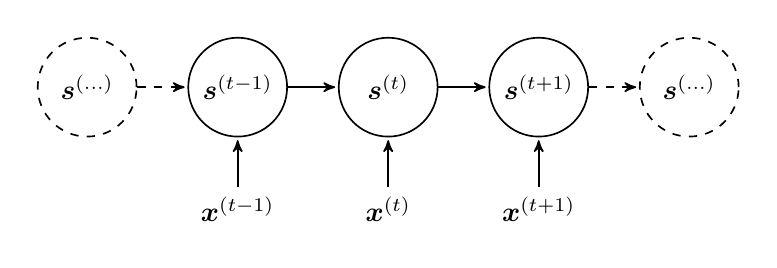
\begin{tikzpicture}[->,>=stealth'
  ,shorten >=1pt
  ,auto
  ,node distance=2.8cm,
  semithick]
  \tikzstyle{every state}=[
  minimum size={10pt+width("$x^{(t-1)}$")}]

  \matrix (m) [matrix of nodes
  ,row sep=.25in,column sep=.25in]
  {
    % 5 s's top row
    \node[state,dashed](sd) {$\vc{s}^{(\ldots)}$};&
    \node[state](stm1) {$\vc{s}^{(t-1)}$};	&
    \node[state](st) {$\vc{s}^{(t)}$}; 		&
    \node[state](stp1) {$\vc{s}^{(t+1)}$};	&
    \node[state,dashed](sd2) {$\vc{s}^{(\ldots)}$};\\
    % 3 xs btm
    &
    \node[     ](xtm1) {$\vc{x}^{(t-1)}$}; 		&
    \node[     ](xt) {$\vc{x}^{(t)}$}; 		&
    \node[     ](xtp1) {$\vc{x}^{(t+1)}$} ;		\\
  };
  
  \path[dashed]  (sd) edge       node {} (stm1);
  \path 
  (xtm1) edge  node {} (stm1)
  (stm1) edge       node {} (st)
  (xt) edge  node {} (st)
  (st) edge       node {} (stp1)
  (xtp1) edge  node {} (stp1);
  \path[dashed] (stp1) edge       node {} (sd2)
  ;
  
\end{tikzpicture}

\end{document}